%==============================================================
%  Figura 5.7 - Arresto dell'azionamento all'apertura del
%  cancello di protezione 3
%  Adattamento in italiano della Figura 5.7 dell'IFA Report 2/2017
%
%  Speculare alla Figura 5.6: qui il pericolo e' un solo azionamento,
%  sorvegliato da piu' cancelli. La fascia grigia isola il solo cancello 3
%  (con logica e azionamento), cioe' cio' che rientra nella funzione
%  di sicurezza in esame; gli altri cancelli restano fuori pur essendo
%  collegati alla stessa linea di comando.
%==============================================================
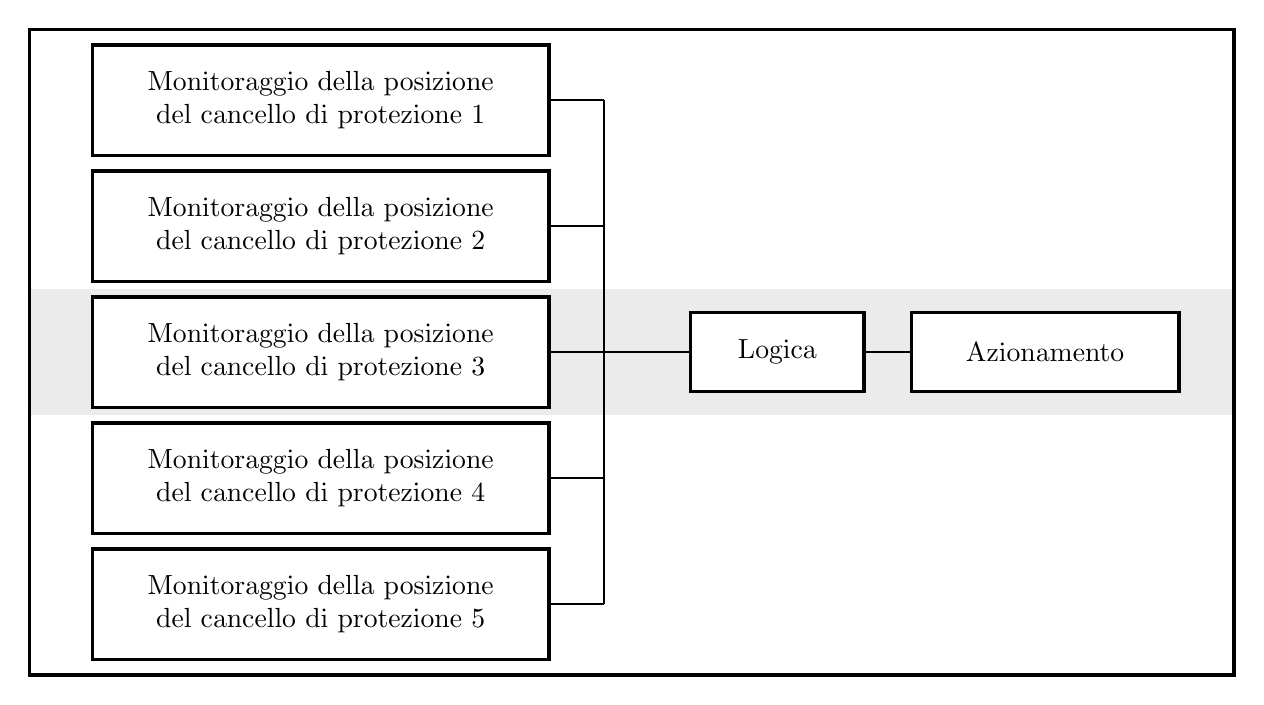
\begin{tikzpicture}[
  font=\normalsize,
  blocco/.style={draw=black, line width=1.2pt, fill=white, align=center,
                 inner sep=4pt, minimum height=1.0cm},
  cancello/.style={blocco, minimum width=5.8cm, minimum height=1.4cm},
  collegamento/.style={draw=black, line width=0.8pt}
]

% Coordinate della cornice, fissate esplicitamente: servono perche' la
% fascia grigia deve attraversare tutta la larghezza del riquadro, come
% nell'originale. Ricavandole dal bounding box si inseguirebbero a vicenda.
\def\cornicesx{-0.70}
\def\cornicedx{14.60}

% ---- campitura: la fascia della funzione di sicurezza --------------
\fill[black!8] (\cornicesx,2.40) rectangle (\cornicedx,4.00);

% ---- blocchi -------------------------------------------------------
\node[cancello] (p1) at (3.0, 6.4) {Monitoraggio della posizione\\del cancello di protezione 1};
\node[cancello] (p2) at (3.0, 4.8) {Monitoraggio della posizione\\del cancello di protezione 2};
\node[cancello] (p3) at (3.0, 3.2) {Monitoraggio della posizione\\del cancello di protezione 3};
\node[cancello] (p4) at (3.0, 1.6) {Monitoraggio della posizione\\del cancello di protezione 4};
\node[cancello] (p5) at (3.0, 0.0) {Monitoraggio della posizione\\del cancello di protezione 5};

\node[blocco, minimum width=2.2cm] (logica)      at (8.8, 3.2) {Logica};
\node[blocco, minimum width=3.4cm] (azionamento) at (12.2,3.2) {Azionamento};

% ---- collegamenti --------------------------------------------------
\draw[collegamento] (6.6,6.4) -- (6.6,0.0);          % linea di raccolta
\draw[collegamento] (p1.east) -- (6.6,6.4);
\draw[collegamento] (p2.east) -- (6.6,4.8);
\draw[collegamento] (p4.east) -- (6.6,1.6);
\draw[collegamento] (p5.east) -- (6.6,0.0);
\draw[collegamento] (p3.east) -- (logica.west);      % cancello 3 -> logica
\draw[collegamento] (logica.east) -- (azionamento.west);

% ---- cornice esterna -----------------------------------------------
\draw[draw=black, line width=1.2pt] (\cornicesx,-0.90) rectangle (\cornicedx,7.30);

\end{tikzpicture}
